\section{习题一 \ DrawBezier}
下面即为绘制代码。
\inputpython{E:/numerical-approximation/code/p3/project3_1.py}{1}{55}
\begin{figure}[hb]
    \centering
    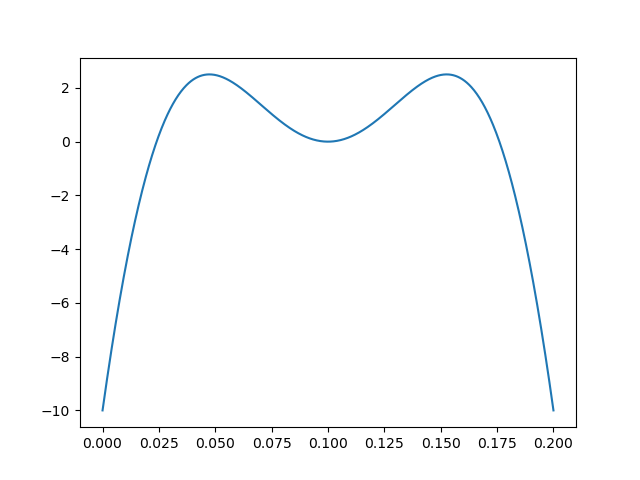
\includegraphics[scale=0.5]{pic/bezier.png}
\end{figure}

\clearpage
\section{习题二 \ 求任意输入t*对应点坐标}
\inputpython{E:/numerical-approximation/code/p3/project3_2.py}{46}{66}
假设输入的t*值为0.01,则在bezier曲线上标注如下图所示。
\begin{figure}[hb]
    \centering
    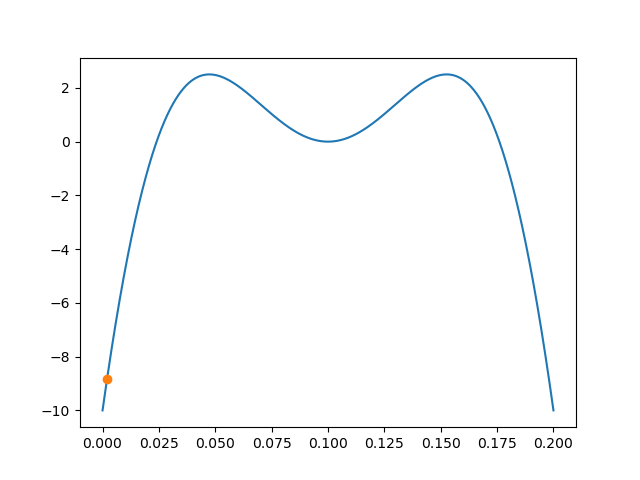
\includegraphics[scale=0.5]{pic/2.png}
\end{figure}

\clearpage
\section{习题三 \ 计算细分曲线控制点}
下面为计算代码。
\inputpython{E:/numerical-approximation/code/p3/project3_3.py}{47}{81}
如下为计算所得x坐标和y坐标数字三角矩阵。
\begin{figure}[htbp]
    \centering
    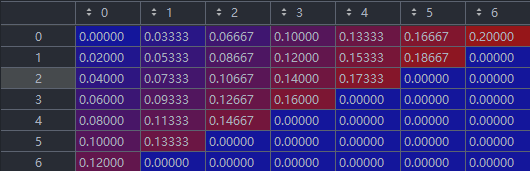
\includegraphics[]{pic/datax.png}
    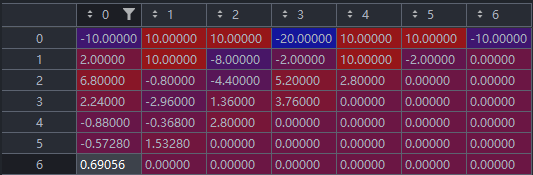
\includegraphics[]{pic/datay.png}
\end{figure}

下图为计算所得的左曲线控制点和右曲线控制点。

\begin{figure}[htbp]
    \centering
    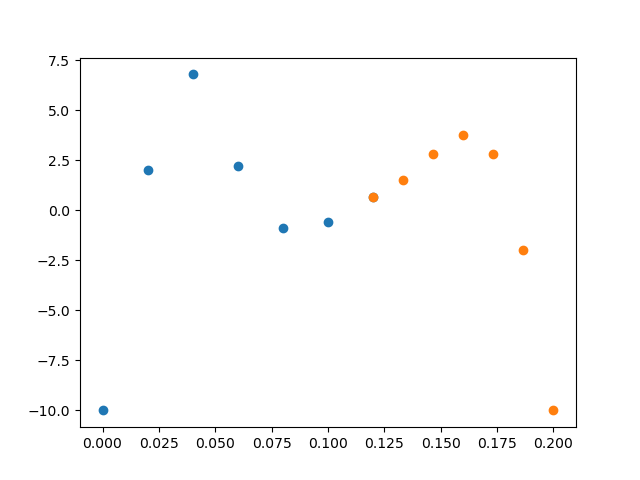
\includegraphics[scale=0.5]{pic/controlpoints.png}
\end{figure}


\clearpage
\section{习题四 \ 升阶算法}
升阶后散点图如下:
\begin{figure}[htbp]
    \centering
    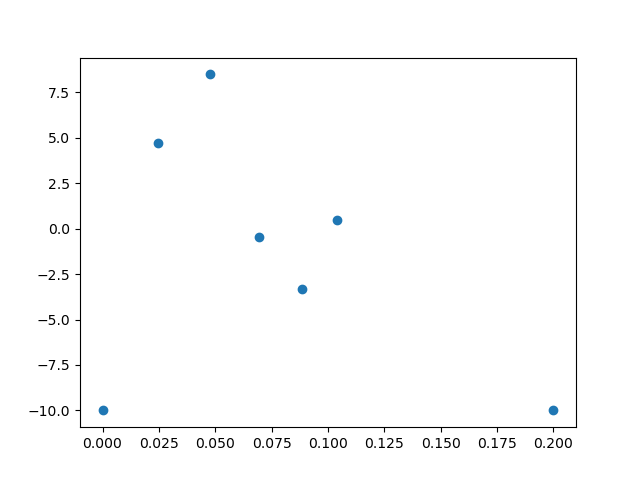
\includegraphics[scale=0.5]{pic/4.png}
\end{figure}
